\documentclass{beamer}
\usepackage{isolatin1}
\usepackage{latexsym}

\usepackage{listings}
\lstset{language=XML,showspaces=false,showtabs=false}

\usepackage[german]{babel}

\usetheme{Berlin}
\mode<presentation>

\title{Integration von RSS mit verteiltem Publish/Subscribe}
\author{Friedemann Zintel}
\date{16. Februar 2006}

\begin{document}
\bibliographystyle{ieeetr}

\begin{frame}

  \titlepage

\end{frame}

\section*{Outline}
\begin{frame}

  \tableofcontents

\end{frame}

\section{Einleitung}

\begin{frame}

  RSS: RDF-Site-Summary, Rich-Site-Summary oder Really-Simple-Syndication?
  \vspace{0.5cm}
  \begin{itemize}
    \item Das am meisten verbreitete Publish/Subscribe-System im Internet
    \item Nicht Push sondern Polling
    \item Von viele Anbietern unterst�tzt
    \item Beispiele: Blogs, Podcasting (anbieten von Medien-Dateien, z.B. mp3)
  \end{itemize}

\end{frame}

\section{�berblick}

\subsection{Publish/Subscribe}
\begin{frame}
  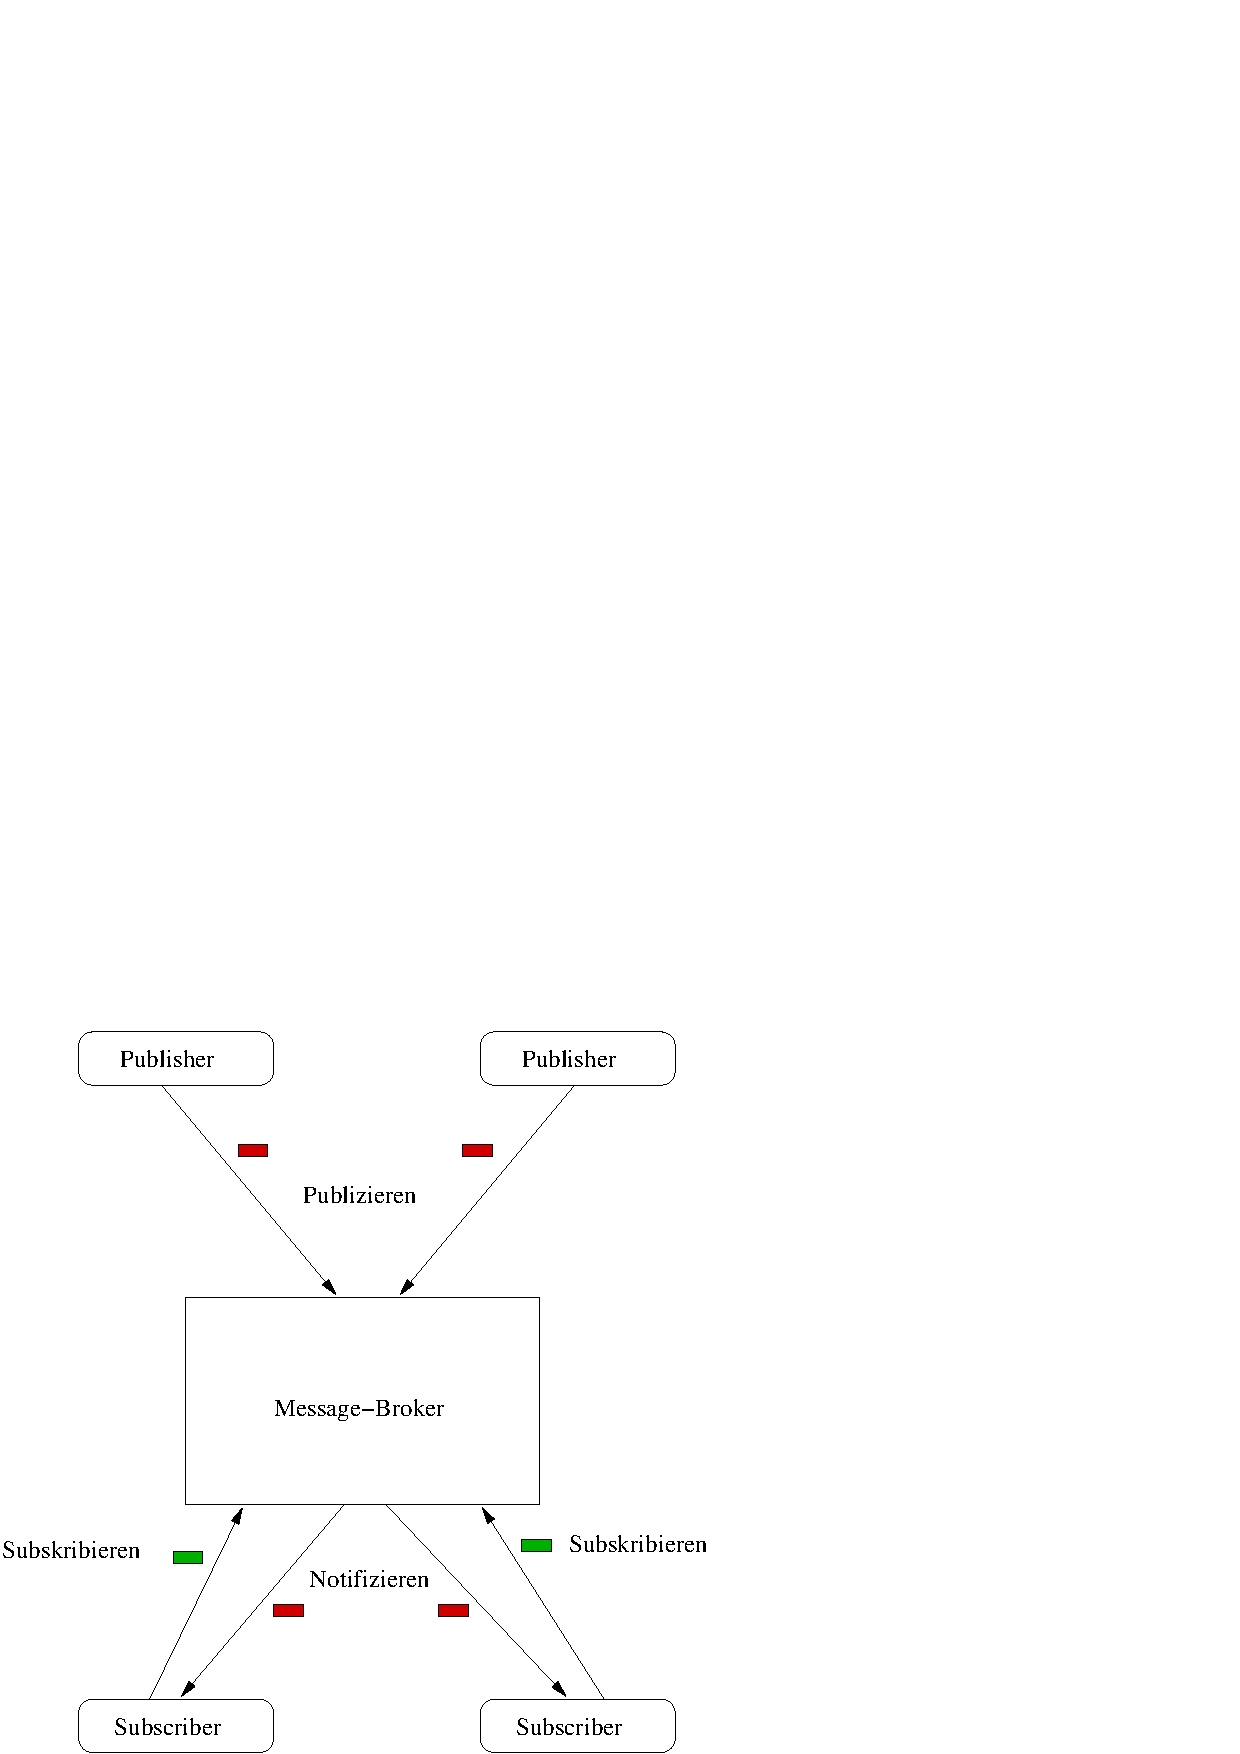
\includegraphics[bb=-50 0 200 350,scale=0.6]{PubSub}
\end{frame}

\subsection{RSS}
\begin{frame}

  \frametitle{RSS}
  \begin{itemize}
    \item RSS-Feed dient u.a. zur Kurzbeschreibung von Web-News
    \item XML-basiert
    \item Erreichbar durch Link auf Anbieterseite oder Angabe in HTML-Head
  \end{itemize}
  \nocite{LiuVenSirer:2005:MeasureRSSPubSub}

\end{frame}

\begin{frame}[fragile,allowframebreaks]
  \frametitle{Beispiel: RSS-Feed}
  \tiny
  \begin{lstlisting}
<?xml version="1.0" encoding="iso-8859-1"?>
<!DOCTYPE rss PUBLIC "-//Netscape Communications//DTD RSS 0.91//EN"
  "http://my.netscape.com/publish/formats/rss-0.91.dtd"> 

<rss version="0.91">

<channel>

 <title>SPIEGEL ONLINE</title>
 <link>http://www.spiegel.de</link>
 <description>Schneller wissen, was wichtig ist</description>
 <language>de</language>

 <image>
  <title>SPIEGEL ONLINE</title>
  <url>http://www.spiegel.de/static/sys/logo_120x61.gif</url>
  <link>http://www.spiegel.de</link>
 </image>
  \end{lstlisting}
  \begin{lstlisting}
 <item>
  <title>Bagdad Sniper:  Der Mann, der Juba &#252;berlebte</title>
  <link>http://www.spiegel.de/panorama/0,1518,394137,00.html</link>
 </item>

 <item>
  <title>Infineon:  Vorstand streitet &#252;ber Speichersparte</title>
  <link>http://www.spiegel.de/wirtschaft/0,1518,394143,00.html</link>
 </item>

 <item>
  <title>Biathlon:  Glagow l&#228;uft Olympiasiegerin davon</title>
  <link>http://www.spiegel.de/sport/wintersport/0,1518,394138,00.html</link>
 </item>

 </channel>
 </rss>
  \end{lstlisting}
  Quelle: www.heise.de
\end{frame}

\section{Motivation}
\begin{frame}

  \frametitle{Anwendersicht: Was man gerne h�tte ...}
  \begin{itemize}
    \item Automatische Benachrichtigung �ber Feed-Updates
    \item Aktualit�t der Feeds
    \item Definition von Filtern auf h�herer Ebene: zur \dots
      \begin{list}{}{}
        \item \dots individuellen Vorselektion der Feeds
	\item \dots anbieter�bergreifenden Auswahl von Feeds
      \end{list}
  \end{itemize}

\end{frame}

\begin{frame}

  \frametitle{Stand der Dinge}
  \begin{itemize}
    \item RSS: Kein push-basiertes Pub/Sub $\rightarrow$ Client/Server
    \item Feeds m�ssen von Anwendersoftware heruntergeladen werden (Polling)
    \item Vordefinierte Channel $\rightarrow$ thematische Zuordnung auf RSS-Server-Seite
    \item Definition von Filtern nur auf Anwenderseite m�glich
  \end{itemize}

  \pause
  Probleme:
  \begin{itemize}
    \item Polling:
      \begin{list}{$\longrightarrow$}{}
        \item Gro�er Datenverkehr im Netz
	\item Hohe server-seitige Last
      \end{list}
    \item Filterdefinition nur beim Anwender:
      \begin{list}{$\longrightarrow$}{}
        \item Alle Feeds m�ssen heruntergeladen werden
      \end{list}
  \end{itemize}
  \nocite{Hicks:2004:RSSBandwith}
  
\end{frame}

\begin{frame}

  \frametitle{Ziel}
  \begin{itemize}
    \item \glqq Entlastung\grqq der RSS-Server
    \item Reduzierung des Datenverkehrs aufgrund von Polling
    \item Erh�hung des Aktualit�tsgrades der Feeds auf Nutzerseite
    \item Erm�glichung der subscriber-seitigen Definition von Filtern
  \end{itemize}

\end{frame}

\section{Umsetzung}
\subsection{Integration von RSS in verteiltes Pub/Sub-System}

\begin{frame}
  \frametitle{Integration von RSS in verteiltes Pub/Sub-System}
  Innerhalb eines Overlay-Netzwerkes wird f�r die Verteilung der Feeds gesorgt.\\
  \vspace{0.5cm}
  Als Grundlage kann eine schon existierende Pub/Sub-Middleware dienen (z.B. REBECA\cite{MuFiBu:2001:ArchFrameECommApp}).
\end{frame}

\begin{frame}
  \vspace{0.5cm}
  \begin{itemize}
    \item RSS-Server k�nnte als Publisher fungieren
    \item Broker sorgen f�r eine Verteilung der Feeds an Nutzer (Subscriber)
  \end{itemize}
  \vspace{0.5cm}

  \pause
  Problem:\\
  Neue Software muss sowohl auf Server-Seite als auch auf Anwenderseite installiert werden.
%    \item Verteilung der RSS-Feeds mittels herk�mmlichem Pub/Sub $\Longrightarrow$ Notifikation der Subscriber
\end{frame}

\begin{frame}
  \frametitle{L�sung:}
\begin{itemize}
  \item Rolle der RSS-Server ver�ndert sich nicht
  \item Nutzer holen Feed in der Rolle des Publisher und speisen ihn in das Broker-Netz
  \item Broker verteilen Feeds an Nutzer bzw. Subscriber
\end{itemize}
\end{frame}

\begin{frame}
  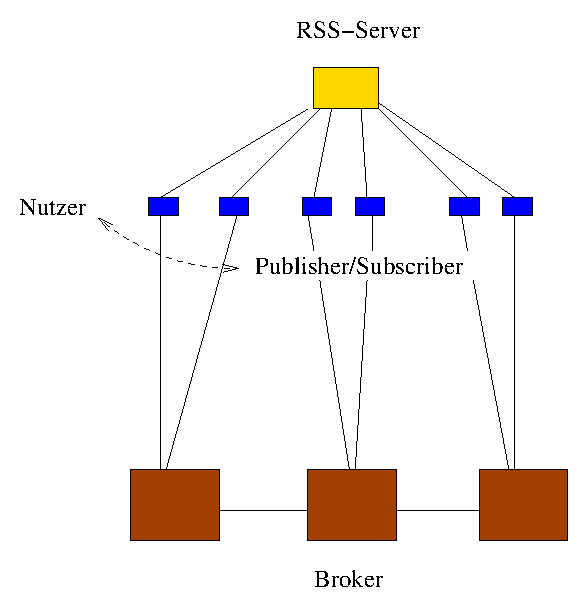
\includegraphics[bb=-100 0 200 250,scale=0.6]{RSSPubSub}
\end{frame}

\begin{frame}
  \frametitle{Ansatz: Ein Publisher}
  \begin{itemize}
    \item Ein Publisher w�rde ausreichen, um Feed herunterzuladen
    \item Alle weiteren Nutzer  bzw. Subscriber w�rden den Feed �bers Netzwerk erhalten
  \end{itemize}

  \pause
  Vorteil:\\
  Wenige Anfragen an den RSS-Server
\vspace{0.5cm}
  
  \pause
  Problem:\\
  Aktualit�t der Feeds!\\
  $\longrightarrow$ lange �bertragungszeiten in Abh�ngigkeit von Netzstruktur\\
  u. U. aufw�ndiger Auswahlprozess\\
  Single Point of Failure
\end{frame}

\begin{frame}
  \frametitle{Aktualit�t vs. Server-Belastung}
  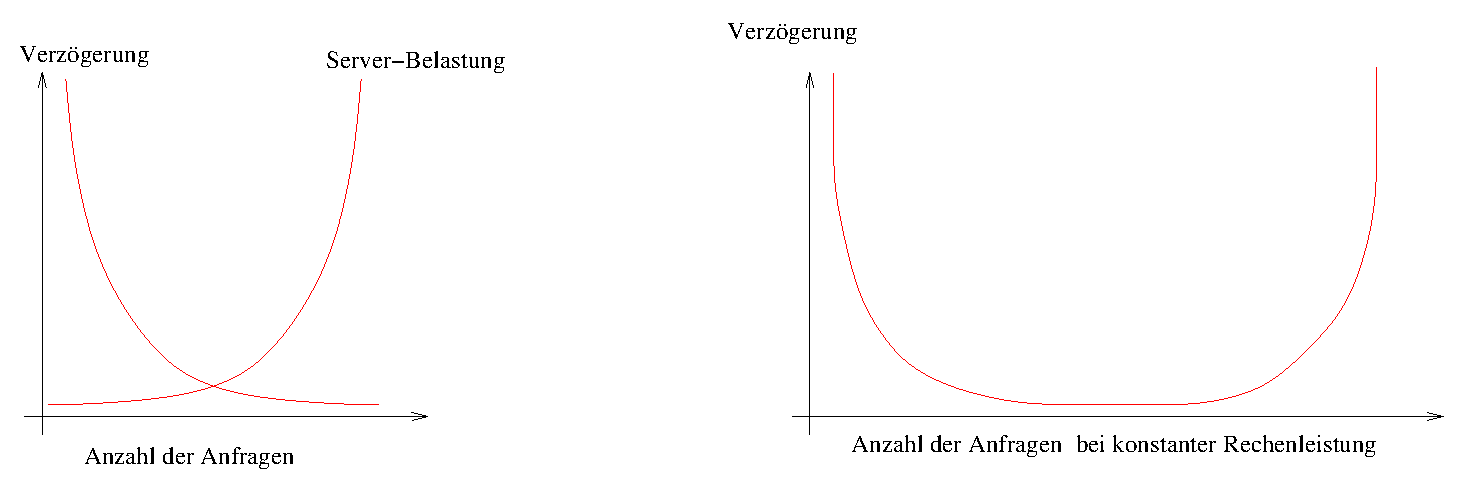
\includegraphics[bb=40 0 200 250,scale=0.5]{Verzoegerung}
\end{frame}

\begin{frame}
  \frametitle{Ansatz: Mehrere Publisher}
  \begin{itemize}
    \item Mehrere Publisher laden Feed herunter
    \item $\rightarrow$ Mindestens so viele, dass gewisse Aktualit�t der Feeds erreicht wird
    \item $\rightarrow$ H�chstens so viele, dass Server nicht �berlastet wird
  \end{itemize}
\vspace{0.5cm}

$\longrightarrow$ Ein optimaler Kompromiss soll erreicht werden

\end{frame}

\begin{frame}
  \frametitle{Frage:}
  Wie k�nnen sich die Publisher dar�ber abstimmen, wer als n�chstes den aktuellen Feed abholt?
\end{frame}

\begin{frame}
  \frametitle{Herausforderungen}
Entwicklung eines bzw. mehrerer Algorithmen zur \dots
  \begin{itemize}
    \item \dots Koordination der Publisher
    \item \dots Ermittlung der RSS-Server-Auslastung
    \item \dots Bestimmung des Update-Intervalls eines Feeds
    \item \dots Bestimmung der Nachrichtenlaufzeiten (eventuell)
  \end{itemize}
\end{frame}

\begin{frame}
  \frametitle{Erwartungen an den Algorithmus}
  Der Entwurf des Algorithmus sollte unter folgenden Gesichtspunkten erfolgen:
  \begin{itemize}
    \item Vermeidung von \glqq Hotspots\grqq
    \item Broker sollen Parameter automatisch einstellen bzw. beziehen
    \item Parameter sollen sich den dynamischen Gegebenheiten des Netzes anpassen
    \item Netz soll auftretende Fehler �berstehen und selbst�ndig beseitigen
  \end{itemize}
\end{frame}

\begin{frame}
  \frametitle{Vorteile des Ansatzes}
  Vorteile gegen�ber �hnlichen Ans�tzen (wie z.B. FeedTree\cite{SandlerEtAl:2005:FeedTree}):
  \begin{itemize}
    \item L�sung kann sich problemlos in bestehende RSS-Architektur integrieren
    \item Bestehende Client-Software kann weiter verwendet werden
    \item Komplette Neukonstruktion eines Pub/Sub-Systems ist nicht notwendig\\
      $\longrightarrow$ in REBECA\cite{MuFiBu:2001:ArchFrameECommApp} sind Filtertechniken bereits integriert
  \end{itemize}
\end{frame}

\section{Literatur}
\begin{frame}[allowframebreaks]
  \bibliography{../bibdatabase}
\end{frame}

\end{document}
